\section{Alternating Finite Automaton(AFA)}

Alternating finite automaton is a generalization of
nondeterminism\cite{Yu1997}. An AFA is equipped with a set of
states, whom we take for a set of propositional variables. In AFA setting,
propositions act as states. Accepting states in NFA are, in turn, propositions
satisfied by a boolean value assignment designated in AFA definition.

\begin{definition}
An alternating finite automaton (AFA) is a 5-tuple \( \mathcal{A} = (Q, s, f,
\Sigma, \delta) \), where \( s \in Q \) is an initial state, \( f \in
\mathcal{B}^Q \) is an accept condition and \( \delta: Q \times \Sigma \times
\mathit{Prop} \) is a transition relation.
\end{definition}

The transition relation \( \delta \) designates a transition to a proposition \(
\alpha \) from a state \( q \) reading an input symbol \( a \), and we write \(
\alpha = \delta(q, a) \) as a shorthand for \( (q, a, \alpha) \in \delta \). In
case a transition has multiple destination propositions, we connect them with
disjunction to have the single destination \( \bigvee \{ \alpha \mid (q, a,
\alpha) \in \delta \} \).

Here we introduce a transition function. The auxiliary function \(
\Delta(\alpha, a) \) performs the simultaneous substitution for each
propositional variable \( q_1, ..., q_n \) in \( \alpha \), \( \Delta(\alpha, a)
:= \alpha[\delta(q_1, a)/q_1 \ ...\ \delta(q_n, a)/q_n] \). Reading each symbol
in a string, \( \hat{ \Delta } \) repetitively substitute the record in \(
\delta \) for the variables: \( (\rm i) \) \( \hat{\Delta}(\alpha, \epsilon) :=
\alpha \) \( (\rm ii) \) \( \hat{\Delta}(\alpha, wa) :=
\Delta(\hat{\Delta}(\alpha, w), a) \).

We write \( \alpha \xrightarrow[]w \beta \) to denote \( \beta =
\hat{\Delta}(\alpha, w) \) and we say a word \( w \) is accepted if \( s
\xrightarrow[]w \alpha \) and \( f \models \alpha \).  The language of \(
\mathit{AFA} \) \( \mathcal{A} \) is defined as \( L(\mathcal{A}) = \{ w \mid
\exists \alpha .\ s \xrightarrow[]w \alpha \wedge f \models \alpha \} \).

\begin{example}
Let AFA \( \mathcal{A} \) have 
states \( \{q_0, q_1, q_2\} \) and whose \( \delta \), \( f \) and \(
s \) be specified below.
\begin{align*}
  \begin{array}{c|cc}
    \delta & a & b \\\hline
    q_0 & q_1 \wedge q_2      & 0              \\
    q_1 & q_2                 & q_1 \wedge q_2 \\
    q_2 & \neg q_1 \wedge q_2 & q_1 \vee \neg q_2
  \end{array}&& f = \begin{smallmatrix}q_0 &\mapsto 0\\q_1 &\mapsto 0\\q_2 &\mapsto 1\end{smallmatrix} && s = q_0
\end{align*}

AFA \( \mathcal{A} \) accepts the string ``\( aa \)''. \(q_0
\xrightarrow[]a q_1 \wedge q_2 \xrightarrow[]a (q_2)
\wedge (\neg q_1 \wedge q_2) \equiv \neg q_1 \wedge q_2 \) and \( f \models \neg
q_1 \wedge q_2 \). Both of ``\(a\)'' and ``\( ab \)'' reach to the identical proposition. \(q_0
\xrightarrow[]a q_1 \wedge q_2 \xrightarrow[]b (q_1 \wedge q_2)
\wedge (q_1 \vee \neg q_2) \equiv q_1 \wedge q_2 \).

\end{example}

\subsection{Construction}

We define construction of AFA along with the structure of a \( \mathit{FOL}
\)-formula \( \varphi \). Given an automatic predicate \( P(x_1, x_2) \), We
define an AFA for a literal \( P \) as \( P = (Q, s, f, \Sigma, \Delta) \). At
this point, we abstract away the ternary relation \( \delta \) in favor of its
functional counterpart \( \Delta \). When combining 2 AFAs \( \mathit{M}_\varphi
\) and \( \mathit{M}_\psi \) along with binary logical connectives, we impose an
assumption on them in left and right hand side that their state sets \(
Q_\varphi \) and \( Q_\psi \) are disjoint and we denote union of them as \(
Q_\varphi \uplus Q_\psi \).  The disjointedness makes sure that union of the 2
valuation functions \( f_\varphi \uplus f_\psi \) is again a well-defined
function and the same applies for \( \delta_\varphi \uplus \delta_\psi \). Note
that except for projection, the input-output relation of \( \delta_{\varphi} \)
remains untouched throughout the construction.

\begin{prooftree}
  \AxiomC{
    \( \mathcal{A}_\varphi = (
    Q_\varphi,
    \Sigma,
    s_\varphi,
    f_\varphi,
    \Delta_\varphi) \)
  }
  \AxiomC{
    \( \mathcal{A}_\psi = (
    Q_\psi,
    \Sigma,
    s_\psi,
    f_\psi,
    \Delta_\psi) \)
  }
  \BinaryInfC{
    \( \mathcal{A}_{\varphi \bigcirc \psi} = (
    Q_\varphi \uplus Q_\psi,
    \Sigma,
    s_\varphi \bigcirc s_\psi,
    f_\varphi \uplus f_\psi,
    \Delta_\varphi \circ \Delta_\psi) \) }
\end{prooftree}

, where \( \bigcirc \) stands for either \( \wedge \) or \( \vee \) and \( \circ
\) is the function composition. Since the application of \( \Delta \) doesn't
change the root symbol, any proposition reachable from \(s_\varphi \wedge s_\psi
\) has \( \wedge \) at its root position. Here we propose \(
L(\mathcal{A}_{\varphi \wedge \psi}) = L(\mathcal{A}_{\varphi}) \cap
L(\mathcal{A}_{\psi}) \) because for any string \( w \in \Sigma^* \), \(
s_\varphi \wedge s_\psi \xrightarrow[]w \varphi' \wedge \psi' \) iff \(
s_\varphi \xrightarrow[]w \varphi' \) and \( s_\psi \xrightarrow[]w \psi' \).

Without loss of generality, we can restrict the domain of \(
\Delta_{\mathcal{A}} \) according to the construction. Suppose \(
\mathcal{A}_{\varphi \wedge \psi} \) is a conjunction of 2 automata \(
\mathcal{A}_{\varphi} \) and \( \mathcal{A}_{\psi} \), then the domain of \(
\Delta_{\varphi \wedge \psi} \) can be restricted to a set of propositions whose
top symbol is \( \wedge \). For arbitrary construction, the following equation
holds.
\begin{align*}
  \Delta_{\varphi \bigcirc \psi}(a, \alpha \bigcirc \beta) &=
  \Delta_\varphi(a, \alpha) \bigcirc \Delta_\psi(a, \beta) \\
  \Delta_{\neg \varphi}(a, \neg \alpha) &= \neg \Delta_\varphi(a, \alpha)
\end{align*}

Quantifiers are represented in terms of the transition function rather than the
tuple structure. Unlike the logical connectives we have seen above, the
quantifiers require us to keep the nested structure. Let \( \mathsf{Q} \) stand
for either \( \forall \) or \( \exists \) and the construction affects none of
the 5-tuple elements.

\[
\Delta_{\forall x_i .\ \varphi}(\mathbf{a}, \alpha) =
\bigwedge\limits_{\mathbf{a}' \in \pi_i(\mathbf{a})} 
\{ \Delta_{\varphi}(\alpha, \mathbf{a}') \}
\quad
\Delta_{\exists x_i .\ \varphi}(\mathbf{a}, \alpha) = 
\bigvee  \limits_{\mathbf{a}' \in \pi_i(\mathbf{a})} 
\{ \Delta_{\varphi}(\alpha, \mathbf{a}') \}
\]

From the induction on the length of strings it follows that
\(L(\mathcal{A}_{\forall x_i .\ \varphi}) = \bigcup\limits_{0 \leq n}\{
\mathbf{w} \in \boldsymbol{\Sigma}^n \mid \text{ for all } w \in \Sigma^n ,
\mathbf{w}[w/i]\in L(\mathcal{A}_{\varphi}) \} \).

\begin{lemma}
Let \(\alpha, \beta \in \mathit{Prop} \). If \( \alpha \Rightarrow \beta \) then for all
\( c \in \Sigma \) \( \Delta(\alpha, c) \Rightarrow \Delta(\beta, c) \).
\end{lemma}

\subsection{Bitencoding, the conversion from DFA to AFA}
\begin{theorem}
[Fella, Jurgensen and Yu] A language \( \mathcal{L} \) is accepted by a DFA with
\( 2^k \) states if and only if it's reversed language \( \mathcal{L}^R \) is
accepted by an AFA with \( k + 1 \) states.
\end{theorem}

\begin{example}
  \begin{figure}
    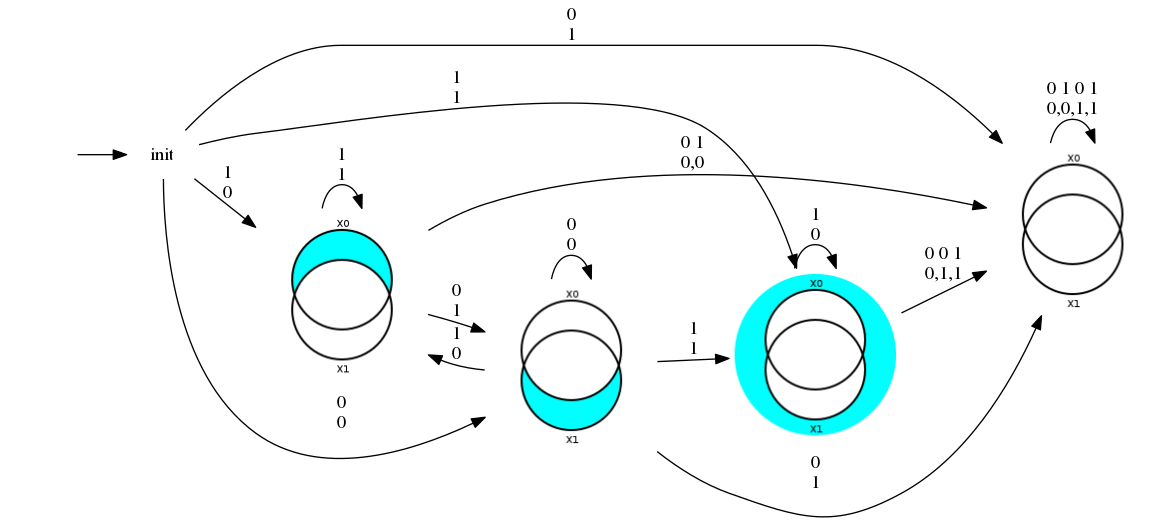
\includegraphics[width=8cm]{images/afa}
  \end{figure}
\end{example}
